\documentclass[a4paper]{quantumarticle}
\pdfoutput=1

\usepackage{lipsum}

\title{Example use of rsmf}

\author{Johannes Jakob Meyer}

\begin{document}
\maketitle

\lipsum[1-10]

\begin{figure}
	\centering
	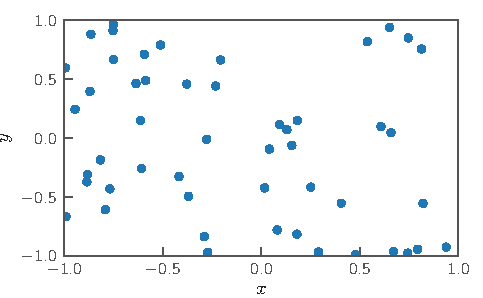
\includegraphics{scatter}
	\caption{\lipsum[2]}
\end{figure}

\lipsum[11-20]

\begin{figure*}
	\centering
	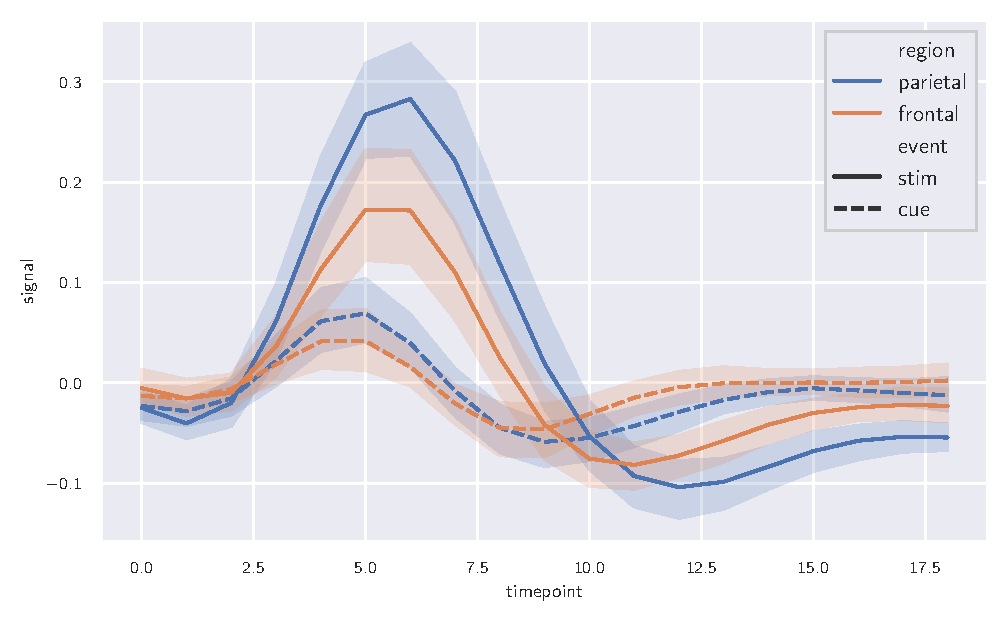
\includegraphics{fmri}
	\caption{\lipsum[1-2]}
\end{figure*}

\lipsum[21-30]

\begin{figure}
	\centering
	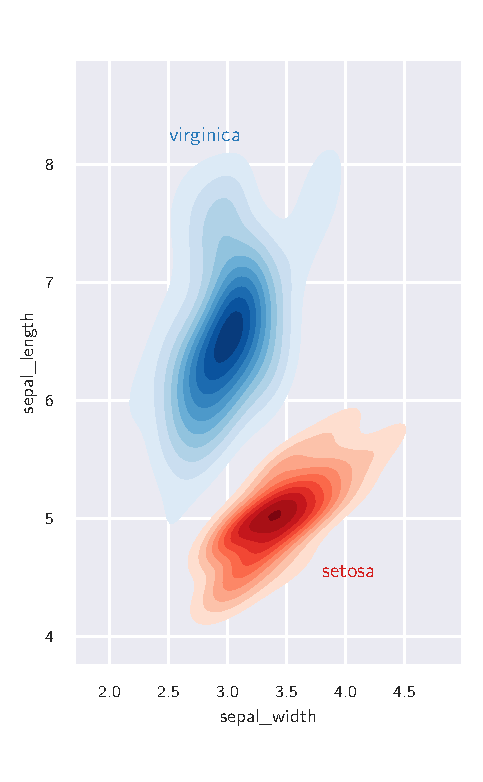
\includegraphics{iris}
	\caption{\lipsum[3]}
\end{figure}

\lipsum[40-50]
    
\end{document}